% Options for packages loaded elsewhere
\PassOptionsToPackage{unicode}{hyperref}
\PassOptionsToPackage{hyphens}{url}
%
\documentclass[
  man,mask,floatsintext]{apa6}
\usepackage{amsmath,amssymb}
\usepackage{iftex}
\ifPDFTeX
  \usepackage[T1]{fontenc}
  \usepackage[utf8]{inputenc}
  \usepackage{textcomp} % provide euro and other symbols
\else % if luatex or xetex
  \usepackage{unicode-math} % this also loads fontspec
  \defaultfontfeatures{Scale=MatchLowercase}
  \defaultfontfeatures[\rmfamily]{Ligatures=TeX,Scale=1}
\fi
\usepackage{lmodern}
\ifPDFTeX\else
  % xetex/luatex font selection
\fi
% Use upquote if available, for straight quotes in verbatim environments
\IfFileExists{upquote.sty}{\usepackage{upquote}}{}
\IfFileExists{microtype.sty}{% use microtype if available
  \usepackage[]{microtype}
  \UseMicrotypeSet[protrusion]{basicmath} % disable protrusion for tt fonts
}{}
\makeatletter
\@ifundefined{KOMAClassName}{% if non-KOMA class
  \IfFileExists{parskip.sty}{%
    \usepackage{parskip}
  }{% else
    \setlength{\parindent}{0pt}
    \setlength{\parskip}{6pt plus 2pt minus 1pt}}
}{% if KOMA class
  \KOMAoptions{parskip=half}}
\makeatother
\usepackage{xcolor}
\usepackage{graphicx}
\makeatletter
\def\maxwidth{\ifdim\Gin@nat@width>\linewidth\linewidth\else\Gin@nat@width\fi}
\def\maxheight{\ifdim\Gin@nat@height>\textheight\textheight\else\Gin@nat@height\fi}
\makeatother
% Scale images if necessary, so that they will not overflow the page
% margins by default, and it is still possible to overwrite the defaults
% using explicit options in \includegraphics[width, height, ...]{}
\setkeys{Gin}{width=\maxwidth,height=\maxheight,keepaspectratio}
% Set default figure placement to htbp
\makeatletter
\def\fps@figure{htbp}
\makeatother
\setlength{\emergencystretch}{3em} % prevent overfull lines
\providecommand{\tightlist}{%
  \setlength{\itemsep}{0pt}\setlength{\parskip}{0pt}}
\setcounter{secnumdepth}{-\maxdimen} % remove section numbering
% Make \paragraph and \subparagraph free-standing
\ifx\paragraph\undefined\else
  \let\oldparagraph\paragraph
  \renewcommand{\paragraph}[1]{\oldparagraph{#1}\mbox{}}
\fi
\ifx\subparagraph\undefined\else
  \let\oldsubparagraph\subparagraph
  \renewcommand{\subparagraph}[1]{\oldsubparagraph{#1}\mbox{}}
\fi
\ifLuaTeX
\usepackage[bidi=basic]{babel}
\else
\usepackage[bidi=default]{babel}
\fi
\babelprovide[main,import]{english}
% get rid of language-specific shorthands (see #6817):
\let\LanguageShortHands\languageshorthands
\def\languageshorthands#1{}
% Manuscript styling
\usepackage{upgreek}
\captionsetup{font=singlespacing,justification=justified}

% Table formatting
\usepackage{longtable}
\usepackage{lscape}
% \usepackage[counterclockwise]{rotating}   % Landscape page setup for large tables
\usepackage{multirow}		% Table styling
\usepackage{tabularx}		% Control Column width
\usepackage[flushleft]{threeparttable}	% Allows for three part tables with a specified notes section
\usepackage{threeparttablex}            % Lets threeparttable work with longtable

% Create new environments so endfloat can handle them
% \newenvironment{ltable}
%   {\begin{landscape}\centering\begin{threeparttable}}
%   {\end{threeparttable}\end{landscape}}
\newenvironment{lltable}{\begin{landscape}\centering\begin{ThreePartTable}}{\end{ThreePartTable}\end{landscape}}

% Enables adjusting longtable caption width to table width
% Solution found at http://golatex.de/longtable-mit-caption-so-breit-wie-die-tabelle-t15767.html
\makeatletter
\newcommand\LastLTentrywidth{1em}
\newlength\longtablewidth
\setlength{\longtablewidth}{1in}
\newcommand{\getlongtablewidth}{\begingroup \ifcsname LT@\roman{LT@tables}\endcsname \global\longtablewidth=0pt \renewcommand{\LT@entry}[2]{\global\advance\longtablewidth by ##2\relax\gdef\LastLTentrywidth{##2}}\@nameuse{LT@\roman{LT@tables}} \fi \endgroup}

% \setlength{\parindent}{0.5in}
% \setlength{\parskip}{0pt plus 0pt minus 0pt}

% Overwrite redefinition of paragraph and subparagraph by the default LaTeX template
% See https://github.com/crsh/papaja/issues/292
\makeatletter
\renewcommand{\paragraph}{\@startsection{paragraph}{4}{\parindent}%
  {0\baselineskip \@plus 0.2ex \@minus 0.2ex}%
  {-1em}%
  {\normalfont\normalsize\bfseries\itshape\typesectitle}}

\renewcommand{\subparagraph}[1]{\@startsection{subparagraph}{5}{1em}%
  {0\baselineskip \@plus 0.2ex \@minus 0.2ex}%
  {-\z@\relax}%
  {\normalfont\normalsize\itshape\hspace{\parindent}{#1}\textit{\addperi}}{\relax}}
\makeatother

\makeatletter
\usepackage{etoolbox}
\patchcmd{\maketitle}
  {\section{\normalfont\normalsize\abstractname}}
  {\section*{\normalfont\normalsize\abstractname}}
  {}{\typeout{Failed to patch abstract.}}
\patchcmd{\maketitle}
  {\section{\protect\normalfont{\@title}}}
  {\section*{\protect\normalfont{\@title}}}
  {}{\typeout{Failed to patch title.}}
\makeatother

\usepackage{xpatch}
\makeatletter
\xapptocmd\appendix
  {\xapptocmd\section
    {\addcontentsline{toc}{section}{\appendixname\ifoneappendix\else~\theappendix\fi\\: #1}}
    {}{\InnerPatchFailed}%
  }
{}{\PatchFailed}
\keywords{Siblings, Lexical Development, Input Effects, Language Acquisition\newline\indent Word count: X}
\usepackage{lineno}

\linenumbers
\usepackage{csquotes}
\ifLuaTeX
  \usepackage{selnolig}  % disable illegal ligatures
\fi
\IfFileExists{bookmark.sty}{\usepackage{bookmark}}{\usepackage{hyperref}}
\IfFileExists{xurl.sty}{\usepackage{xurl}}{} % add URL line breaks if available
\urlstyle{same}
\hypersetup{
  pdftitle={Analysing the effect of sibling number on input and output in the first 18 months: Supplementals},
  pdflang={en-EN},
  pdfkeywords={Siblings, Lexical Development, Input Effects, Language Acquisition},
  hidelinks,
  pdfcreator={LaTeX via pandoc}}

\title{Analysing the effect of sibling number on input and output in the first 18 months: Supplementals}
\author{\textsuperscript{1} \& \textsuperscript{2}}
\date{}


\shorttitle{Effect of sibling number on language: Supplementals}

\authornote{

Correspondence concerning this article should be addressed to , . E-mail:

}

\affiliation{\vspace{0.5cm}\textsuperscript{1} \\\textsuperscript{2} }

\begin{document}
\maketitle

The supplementary materials below present further analyses on our sample. We include this data here for sake of completeness and transparency, but do not include it in the reported results owing to small sample sizes and consistency across findings. All scripts and data for our analysis can be found on the project's OSF wiki at \url{https://osf.io/rm3ec/}.

The analyses below (S1:S8) show:

\begin{itemize}
\tightlist
\item
  S1: re-analysis of caregiver input variables using data from day-long audio recordings
\item
  S2: re-analysis of caregiver input variables with both dizygotic twins excluded
\item
  S3: summary of speakers classed as two main caregivers in our input data
\item
  S4: correlations of input and output measures with maternal factors (age, education, work status) and number of siblings
\item
  S5: re-analysis of caregiver input variables using discrete sibling number as our main variable of interest
\item
  S6: re-analysis of caregiver input variables with one outlier infant
\item
  S7: change to input variables over time
\item
  S8: validating CDI scores with infant productions in the home-recorded data
\end{itemize}

Consistent with our main analysis, all analyses here draw on data from age 10 months, given that the majority of infants did not produce their first word until around 0;11, according to CDI reports. In addition, the twin removed from the main analyses is also removed from the data analysed here.

\hypertarget{s1-effect-of-siblings-on-infants-input---audio-recordings}{%
\subsection{S1: Effect of siblings on infants' input - audio recordings}\label{s1-effect-of-siblings-on-infants-input---audio-recordings}}

Our main results analyse input data from the hour-long video recordings taken in the home on a monthly basis. We opted to use the video data in the main analysis due to consistency in data collection across time-points (one hour of video recording per month, per child). We re-ran our analysis using the home-recorded audio data, which captures a snapshot from a 16h daylong recording using a LENA device (\url{https://www.lena.org/}) worn in a vest. Three or four hours were transcribed per monthly recording; four hours in the 10-13-month recordings, and three hours in the 14-17-month recordings. These transcribed sections were selected based on the most talkative hours in each recording, as determined by an algorithm that ranked hour-long subregions according to LENA's CVC and CTC metrics over the entire 16h recording.

Initial model comparisons including the caregiver input/object presence as a dependent variable and age and sex as fixed effects showed no effect for sex on either measure, but an effect of age on both. Age, but not sex, was thus included in our regression models; data was included from age 10 months onwards.

We tested our two input variables using nested model comparisons, where (1) is the baseline model and (2) includes siblings as the variable of interest.

\begin{enumerate}
\def\labelenumi{\arabic{enumi}.}
\tightlist
\item
  caregiver input/object presence (log-transformed) \textasciitilde{} age (months) + (1\textbar subject)
\item
  caregiver input/object presence (log-transformed) \textasciitilde{} sibling group + age (months) + (1\textbar subject)
\end{enumerate}

Outputs from these model comparisons and full model outputs including estimates are shown in Tables \ref{tab:table-model-comparisons-audio} and \ref{tab:table-input-model-summary-audio}. Results were consistent with the video data for object presence, where a significant effect was found for sibling group. Unlike the video data, this effect was not found in the model testing overall input.

\begin{longtable}[t]{ccccc}
\caption{\label{tab:table-model-comparisons-audio}Results of nested model comparisons testing the effect of sibling group on caregiver input/object presence in the audio data. Linear mixed-effects regression models compared our two input measures (object words produced in caregiver input  and object presence) in relation to sibling group (0 vs. 1 vs. 2+) in the audio data. Age in months was included as a fixed effect; subject was included as a random effect.}\\
\toprule
Model & Df & Chisq & p value & $R^{2}$\\
\midrule
Caregiver input & 2 & 2.75 & 0.252 & 0.69\\
Object presence & 2 & 19.49 & <0.001 & 0.44\\
\bottomrule
\end{longtable}

\begin{longtable}[t]{ccccccc}
\caption{\label{tab:table-input-model-summary-audio}Full model outputs from two linear mixed effects regression models comparing our input measures (object words produced in caregiver input and object presence) in relation to sibling group (0 vs. 1 vs. 2+), for the audio data. Age in months was included as a fixed effect in both models and subject was included as a random effect.}\\
\toprule
Variable & Effect & Estimate & Std. Error & df & t value & p value\\
\midrule
Caregiver input & Intercept & 5.24 & 0.18 & 168.09 & 29.34 & <0.001\\
 & SibGroupOne & 0.12 & 0.20 & 43.00 & 0.62 & 0.539\\
 & SibGroup2+ & -0.28 & 0.22 & 43.00 & -1.27 & 0.212\\
 & month & 0.03 & 0.01 & 301.00 & 2.97 & 0.003\\
\midrule
Object presence & Intercept & 0.38 & 0.04 & 341.20 & 8.50 & <0.001\\
\addlinespace
 & SibGroupOne & -0.09 & 0.03 & 43.00 & -3.11 & 0.003\\
 & SibGroup2+ & -0.15 & 0.03 & 43.00 & -4.69 & <0.001\\
 & month & 0.02 & 0.00 & 301.00 & 6.46 & <0.001\\
\bottomrule
\end{longtable}

\newpage

\hypertarget{s2-re-analysis-of-caregiver-input-variables-with-both-dizygotic-twins-excluded}{%
\subsection{S2: re-analysis of caregiver input variables with both dizygotic twins excluded}\label{s2-re-analysis-of-caregiver-input-variables-with-both-dizygotic-twins-excluded}}

As stated in the main paper, there was one pair of dizygotic twins in the original dataset. We retain one infant in the main analysis in order to maximise sample size, but we acknowledge that this is not a perfect solution given that the presence of another twin in the home (counted as a sibling in the main analysis) may affect caregiver interactions in a different way than the presence of an older sibling. By removing both twins from our data and re-analysing the input measures, we can confirm that our results were consistent with and without one of the twins included in our data (n=42). See Tables \ref{tab:table-model-comparisons-no-twins} and \ref{tab:table-input-model-summary-no-twins}.

\begin{longtable}[t]{ccccc}
\caption{\label{tab:table-model-comparisons-no-twins}Results of nested model comparisons testing the effect of sibling group on caregiver input/object presence in the video data, with both dizygotic twins removed from our sample (n=42). Linear mixed-effects regression models compared our two input measures (object words produced in caregiver input  and object presence) in relation to sibling group. Age in months was included as a fixed effect for both models; subject was included as a random effect.}\\
\toprule
Model & Df & Chisq & p value & $R^{2}$\\
\midrule
Caregiver input & 2 & 8.41 & 0.015 & 0.58\\
Object presence & 2 & 27.93 & <0.001 & 0.55\\
\bottomrule
\end{longtable}

\begin{longtable}[t]{ccccccc}
\caption{\label{tab:table-input-model-summary-no-twins}Full model output from linear mixed effects regression models comparing our two input measures (object words produced in caregiver input and object presence) over time in relation to sibling group, with both dizygotic twins removed from our sample (n=42). Age in months was included as a fixed effect in both models; subject was included as a random effect.}\\
\toprule
Variable & Effect & Estimate & Std. Error & df & t value & p value\\
\midrule
Caregiver input & Intercept & 4.77 & 0.16 & 252.93 & 28.95 & <0.001\\
 & SibGroupOne & -0.01 & 0.15 & 42.00 & -0.09 & 0.930\\
 & SibGroup2+ & -0.49 & 0.17 & 42.00 & -2.91 & 0.006\\
 & month & 0.03 & 0.01 & 294.00 & 2.95 & 0.003\\
\midrule
Object presence & Intercept & 0.56 & 0.05 & 316.86 & 12.44 & <0.001\\
\addlinespace
 & SibGroupOne & -0.14 & 0.03 & 42.00 & -3.98 & <0.001\\
 & SibGroup2+ & -0.22 & 0.04 & 42.00 & -5.92 & <0.001\\
 & month & 0.01 & 0.00 & 294.00 & 3.05 & 0.003\\
\bottomrule
\end{longtable}

\newpage

\hypertarget{s3-speakers-in-the-dataset}{%
\subsection{S3: Speakers in the dataset}\label{s3-speakers-in-the-dataset}}

The table below provides a summary of which two caregivers produced the most words in each video recording analyzed in the main manuscript. This was usually the mother and/or the father. In the case where the infant had two mothers, their data was aggregated into the `Mother' category; in four sessions from this family, the two mothers were the two main caregivers. There were 344 hour-long video recordings in total across the 43 infants in the data set; two speakers were present in 148 of these.

\begin{longtable}[t]{ccc}
\caption{\label{tab:table-speakers-sessions}Numer of sessions in which each adult speaker is one of the two main caregivers. There were 344 hour-long video sessions in total, and two caregivers were present in 146 of these.}\\
\toprule
Speaker & Caregiver 1 & Caregiver 2\\
\midrule
Mother & 282 & 16\\
Father & 45 & 83\\
Grandmother & 11 & 24\\
Babysitter & 4 & 4\\
Grandfather & 1 & 5\\
\addlinespace
Other Adult & 1 & 7\\
Aunt & 0 & 7\\
Uncle & 0 & 2\\
\bottomrule
\end{longtable}

\newpage

\hypertarget{s4-correlations-with-maternal-factors}{%
\subsection{S4: Correlations with maternal factors}\label{s4-correlations-with-maternal-factors}}

We tested the extent to which maternal factors such as age, work status and education level correlate with number of siblings, productive vocabulary measures, and amount of input. Spearman's correlation tests confirmed a significant negative correlation between sibling number and words produced in the infant's input by the mother (rho=-0.36, \emph{p}=.028). No other correlations were significant, though weak positive correlations were identified between amount of input and productive vocabulary, maternal age and sibling number, and maternal work hours and education. See Figure \ref{fig:Figure-correlations}.

\begin{figure}
\centering
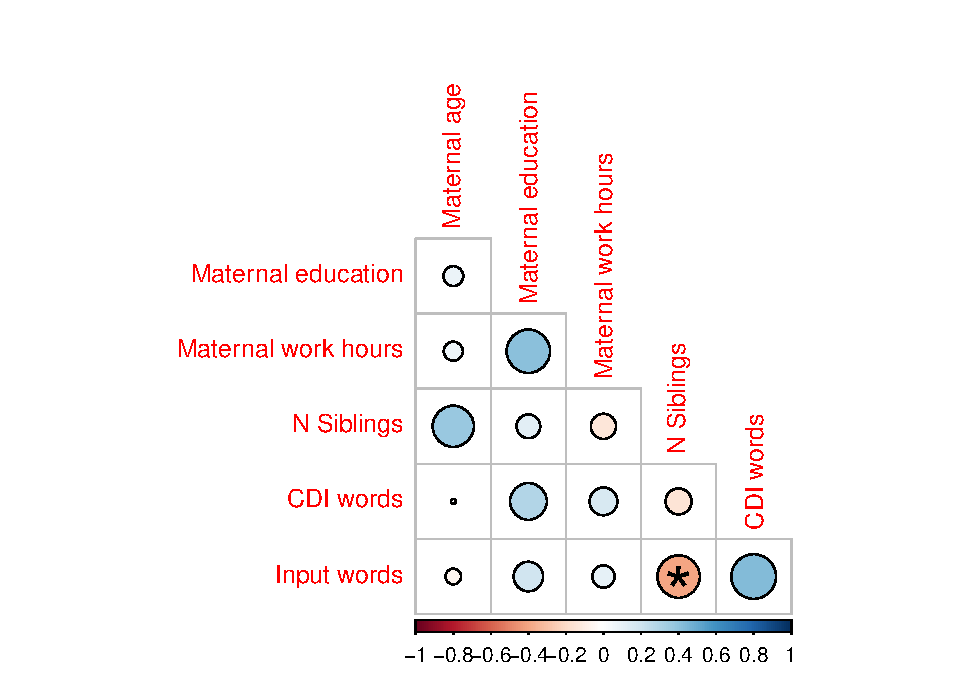
\includegraphics{SiblingsStudy_SupplementaryData-anon-revisions_files/figure-latex/Figure-correlations-1.pdf}
\caption{\label{fig:Figure-correlations}Correlation matrix showing Spearman's correlation coefficients between maternal factors (age, work status and education), number of siblings, and number of words reported to be produced by the child at age 18 months. Colours and circles represent direction and strength of correlation, whereby bolder colours and larger circles indicate a stronger correlation between variables; blue and red indicate positive/negative correlations, respectively. Asterisk indicates a significant \emph{p} value at \emph{p}\textless.05.}
\end{figure}

\newpage

\hypertarget{s5-discrete-sibling-number}{%
\subsection{S5: Discrete sibling number}\label{s5-discrete-sibling-number}}

Our main analyses report the effects of sibling group (infants with 0, 1 or 2+ siblings) on our two input measures (number of input words produced by caregivers and object presence). We opted to go with this measure of sibling number owing to more balanced group sizes. Since discrete sibling number (raw number of siblings) also revealed siblings to be a significant predictor of vocabulary size at 18 months, here we re-run our input models using discrete sibling number as a fixed effect, instead of sibling group, to test whether this effect is consistent across our input measures.

Once again, initial model comparisons including the caregiver input/object presence as a dependent variable and age/sex as fixed effects showed no effect for sex on either measure, but an effect of age on both. Age, but not sex, was thus included in our regression models; data was included from age 10 months on-wards. As above, we tested our two input variables using nested model comparisons, where (1) is the baseline model and (2) includes siblings as the variable of interest.

\begin{enumerate}
\def\labelenumi{\arabic{enumi}.}
\tightlist
\item
  caregiver input/object presence (log-transformed) \textasciitilde{} age (months) + (1\textbar subject)
\item
  caregiver input/object presence (log-transformed) \textasciitilde{} sibling number + age (months) + (1\textbar subject)
\end{enumerate}

Outputs from model comparisons and full model outputs including estimates are shown in Tables \ref{tab:table-model-comparisons-discrete} and \ref{tab:table-input-model-summary-discrete}. Results were consistent with those reported for sibling group, suggesting both characterizations of siblinghood capture similar relationships among our variables.

\begin{longtable}[t]{ccccc}
\caption{\label{tab:table-model-comparisons-discrete}Results of nested model comparisons testing the effect of discrete sibling number on caregiver input/object presence in the video data. Linear mixed-effects regression models compared our two input measures (object words produced in caregiver input  and object presence) in relation to sibling number (R = 0-4). Age in months was included as a fixed effect; subject was included as a random effect.}\\
\toprule
Model & Df & Chisq & p value & $R^{2}$\\
\midrule
Caregiver input & 1 & 5.45 & 0.020 & 0.59\\
Object presence & 2 & 30.24 & <0.001 & 0.55\\
\bottomrule
\end{longtable}

\begin{longtable}[t]{ccccccc}
\caption{\label{tab:table-input-model-summary-discrete}Full model outputs from two linear mixed effects regression models comparing our input measures (object words produced in caregiver input and object presence) in relation to discrete sibling number (R = 0-4), for the video data. Age in months was included as a fixed effect in both models and subject was included as a random effect.}\\
\toprule
Variable & Effect & Estimate & Std. Error & df & t value & p value\\
\midrule
Caregiver input & Intercept & 4.81 & 0.16 & 274.49 & 30.17 & <0.001\\
 & n Siblings & -0.15 & 0.06 & 43.00 & -2.41 & 0.020\\
 & month & 0.03 & 0.01 & 301.00 & 2.95 & 0.003\\
\midrule
Object presence & Intercept & 0.55 & 0.04 & 328.64 & 12.41 & <0.001\\
 & n Siblings & -0.08 & 0.01 & 43.00 & -5.32 & <0.001\\
\addlinespace
 & month & 0.01 & 0.00 & 301.00 & 2.93 & 0.004\\
\bottomrule
\end{longtable}

\newpage

\hypertarget{s6-possible-outlier-for-input-data-removed}{%
\subsection{S6: Possible outlier for input data removed}\label{s6-possible-outlier-for-input-data-removed}}

One infant heard substantially more (\textgreater3SDs above the mean) nouns in their input and nouns with object presence than the other 42 infants in the main sample for four of their recording sessions. We retain this infant in the main analysis, but confirm here that results reported for sibling group were consistent when this child was removed from the analysis of input data (n=42). See Tables \ref{tab:table-model-comparisons-red} and \ref{tab:table-input-model-summary-red}.

\begin{longtable}[t]{ccccc}
\caption{\label{tab:table-model-comparisons-red}Results of nested model comparisons testing the effect of sibling group on caregiver input/object presence in the video data, with one infant identified as an outlier removed from our sample (n=42). Linear mixed-effects regression models compared our two input measures (object words produced in caregiver input  and object presence) in relation to sibling group. Age in months was included as a fixed effect; subject was included as a random effect.}\\
\toprule
Model & Df & Chisq & p value & $R^{2}$\\
\midrule
Caregiver input & 2 & 9.01 & 0.011 & 0.56\\
Object presence & 2 & 26.06 & <0.001 & 0.55\\
\bottomrule
\end{longtable}

\begin{longtable}[t]{ccccccc}
\caption{\label{tab:table-input-model-summary-red}Full model output from linear mixed effects regression models comparing our two input measures (object words produced in caregiver input and object presence) over time in relation to sibling group, with one infant removed who was identified as an outlier (n=42). Age in months was included as a fixed effect in both models, and subject was included as a random effect.}\\
\toprule
Variable & Effect & Estimate & Std. Error & df & t value & p value\\
\midrule
Caregiver input & Intercept & 4.73 & 0.16 & 262.71 & 28.89 & <0.001\\
 & SibGroupOne & 0.08 & 0.14 & 42.00 & 0.54 & 0.593\\
 & SibGroup2+ & -0.44 & 0.16 & 42.00 & -2.74 & 0.009\\
 & month & 0.03 & 0.01 & 294.00 & 2.84 & 0.005\\
\midrule
Object presence & Intercept & 0.56 & 0.05 & 312.10 & 12.26 & <0.001\\
\addlinespace
 & SibGroupOne & -0.12 & 0.03 & 42.00 & -3.67 & <0.001\\
 & SibGroup2+ & -0.22 & 0.04 & 42.00 & -5.74 & <0.001\\
 & month & 0.01 & 0.00 & 294.00 & 3.02 & 0.003\\
\bottomrule
\end{longtable}
\newpage

\hypertarget{s7-change-to-input-variables-over-time}{%
\subsection{S7: Change to input variables over time}\label{s7-change-to-input-variables-over-time}}

We re-plotted Figures 2 and 3 from the main paper with age on the x-axis, to determine whether there was any notable age-related changes in these variables.

\begin{figure}
\centering
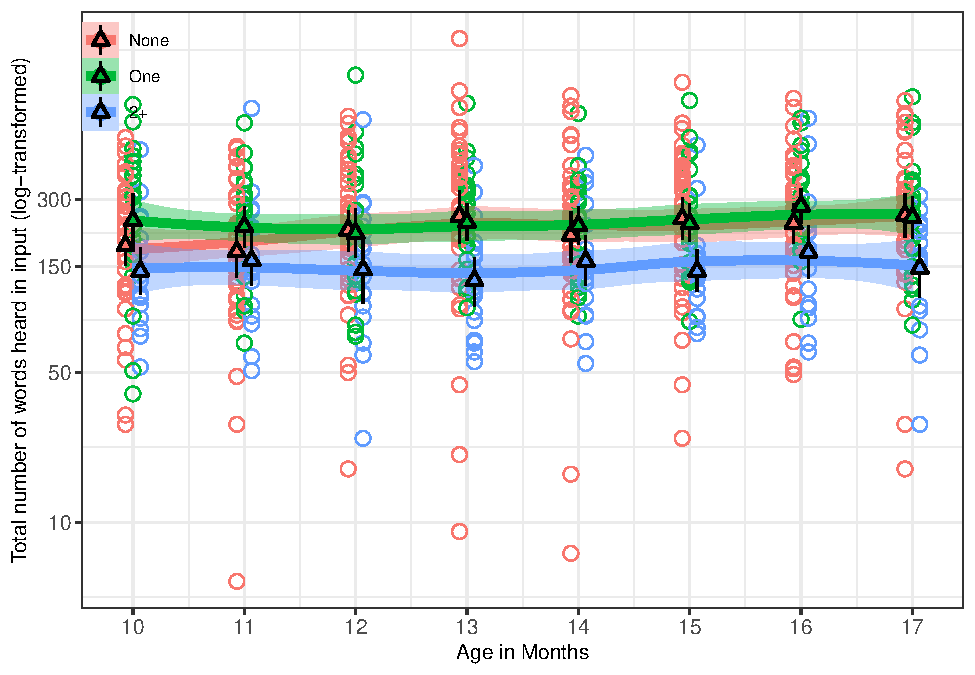
\includegraphics{SiblingsStudy_SupplementaryData-anon-revisions_files/figure-latex/Figure-input-age-1.pdf}
\caption{\label{fig:Figure-input-age}Number of input words produced by caregivers over time (n=43). Colors denote sibling group; line with colored confidence band reflects local estimator (loess) fit over individual infants' input at each month. Triangles indicate mean with bootstrapped CIs computed over each month's data. Points (dodged horizontally for visual clarity) show individual infants' input at each month.}
\end{figure}

\begin{figure}
\centering
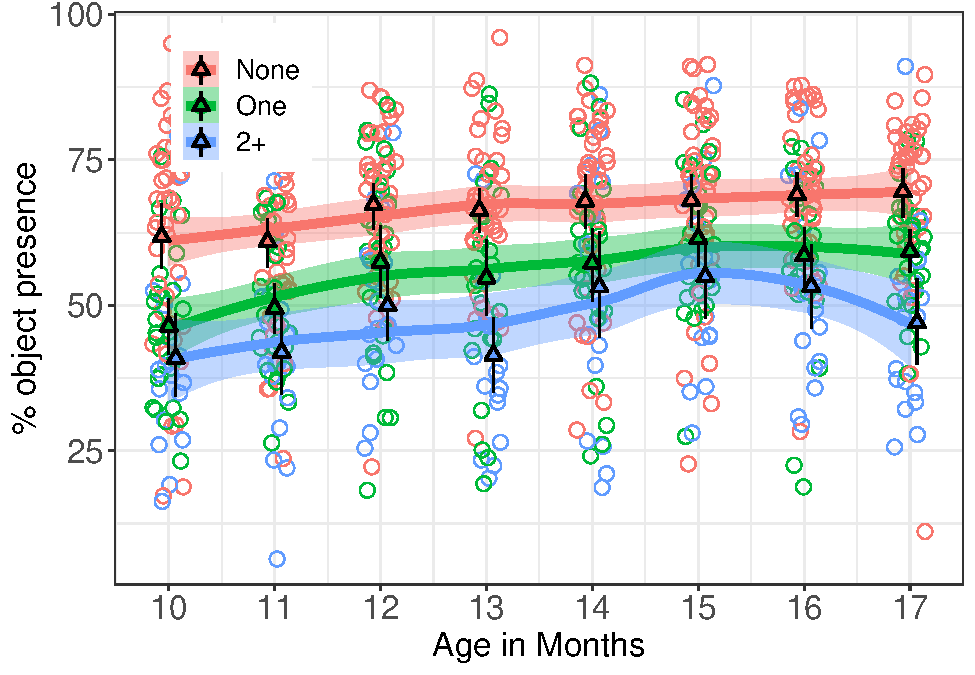
\includegraphics{SiblingsStudy_SupplementaryData-anon-revisions_files/figure-latex/Figure-OP-age-1.pdf}
\caption{\label{fig:Figure-OP-age}Amount (\%) of object presence in infants' input over time (n=43). Colors denote sibling group; line with colored confidence band reflects local estimator (loess) fit over object presence at each month. Triangles indicate mean with bootstrapped CIs computed over each month's data. Points (dodged horizontally for visual clarity) show object presence in individual infants' inputs at each month.}
\end{figure}

Inspection of both Figures \ref{fig:Figure-input-age} and \ref{fig:Figure-OP-age} suggest that both measures were relatively consistent in the data over time, across each sibling group.

\newpage

\hypertarget{s8-validating-cdi-scores-with-infant-productions-in-the-home-recorded-data}{%
\subsection{S8: Validating CDI scores with infant productions in the home-recorded data}\label{s8-validating-cdi-scores-with-infant-productions-in-the-home-recorded-data}}

Parents with more children may have been less aware of the variety of words that their infant could produce, owing to having less time and attention capacity to closely observe their infant's word production. To test the reliability of the reported CDI data used in our analysis, we draw on infants' word production in the home-recorded data (video and audio recordings). Figure \ref{fig:Figure-cdi-types} shows positive correlations between reported productive vocabulary size (CDI) at 18 months and total number of word types produced by the infants in the video and audio recordings by 17 months. Outcomes from Pearson correlation tests are shown in Table \ref{tab:production-corrs}; correlations are positive across all groups, but only significant in the One and None groups, likely owing to the small sample size (n=7) in the 2+ group.

\begin{figure}
\centering
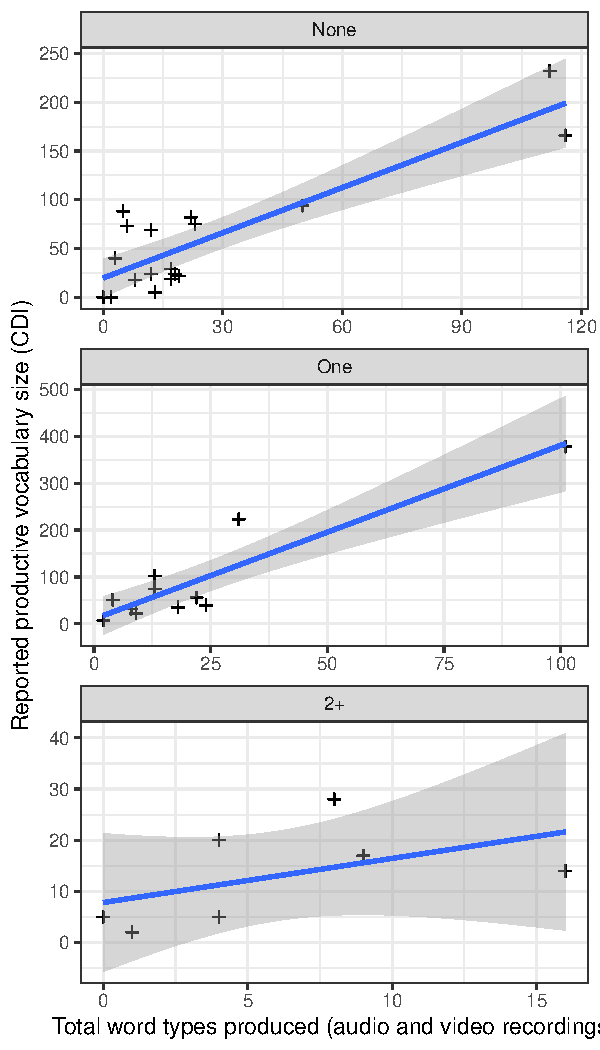
\includegraphics{SiblingsStudy_SupplementaryData-anon-revisions_files/figure-latex/Figure-cdi-types-1.pdf}
\caption{\label{fig:Figure-cdi-types}Correlation between reported productive vocabulary at 18 months and n word types produced in the audio and video recordings at 10-17 months (n=43), faceted by sibling group. Crosses represent individual participants in each sibling group, blue lines represent the predicted relationship between the two variables with 95\% confident intervals for each group. Due to missing CDIs at 18 months, this includes data from n = 18/21, 11/12, and 7/9 children with 0, 1, and 2+ siblings, respectively.}
\end{figure}

\begin{longtable}[t]{cccc}
\caption{\label{tab:production-corrs}Pearson correlation coefficients (r) and p values of correlations between reported productive vocabulary (CDI) at 18 months and number of words produced by infants in the audio/video recordings between 10 and 17 months across sibling groups.}\\
\toprule
SibGroup & n & r & p value\\
\midrule
None & 18 & 0.87 & <0.001\\
One & 11 & 0.92 & <0.001\\
2+ & 7 & 0.50 & 0.259\\
\bottomrule
\end{longtable}


\end{document}
